\subsection{Concept}
The goal of this experiment is to assess efficiency of different reference strategies in Rust, borrowing and reference counting. 

By levaraging reference counting, a value can be shared like what borrowing plays the role in Rust programming. 
The difference is that reference counting checks number of reference pointing to the actual data and makes sure the data is not deleted 
until all the references are dereferenced. Using reference counting is sometimes preferable approach for developers, 
we do not have care about lifetime which is usually troublesome when we use borrowing approach many times in our code. 
However, the possible problem regarding to reference counting is the cost for tracking the number of references. 
Having this assumption, this experiment will show difference of behavior among reference countinig and borrowing.

In this experiment, CustomerBorrowed and CustomerRc in figure are used to see difference of dropping time among borrowing and reference counting. 
In the CustomerRc and OrderRc struct, all fields take reference counting (Rc$<$T$>$). Similaly to the experiment in the last section, 
vectors of CustomerRc and CustomerBorrowed are created and droped the elements one by one. 

The result shows significant difference of dropping time among the two objects; deletion of CustomerRc is much slower than CustomerBorrowed. 
This is because reference counters which are feilds of CustomerRc have to check the number of reference pointing to the actual content and decide 
deallocate the memory or not. However, memory management and lifetime strategy of borrowing is already determined at compile time.


In this experiment, an assessment is conducted to valify whether there is difference between behavior of borrowing and reference counting. 
These two methods can be used in similar situation. Especially, when we want reference to an original variable and keep the original variable until all of references are dereferenced, 
we can have reference with both storategies, borrowing and reference counting. One advantage of using reference counting is that we do not have to pay attention to lifetime.
However, the assumption here is that use of reference counting might be computationally expenesive than borrowing, because reference counting has to track the number of reference pointing to the value. 
Considered this assumption, we assess difference of time for dropping reference using borrowing and reference counting strategies. 

Similally to the last section, we implement struct whose fields are borrowing reference and reference counting and measure the time to drop the struct. 


\subsection{Result}
The result shows the time to drop borrowing reference is significatly faster than reference counting. This says that we should use borrwoing storategies whenever high performance computation is critical.
\begin{figure}[htb!]
    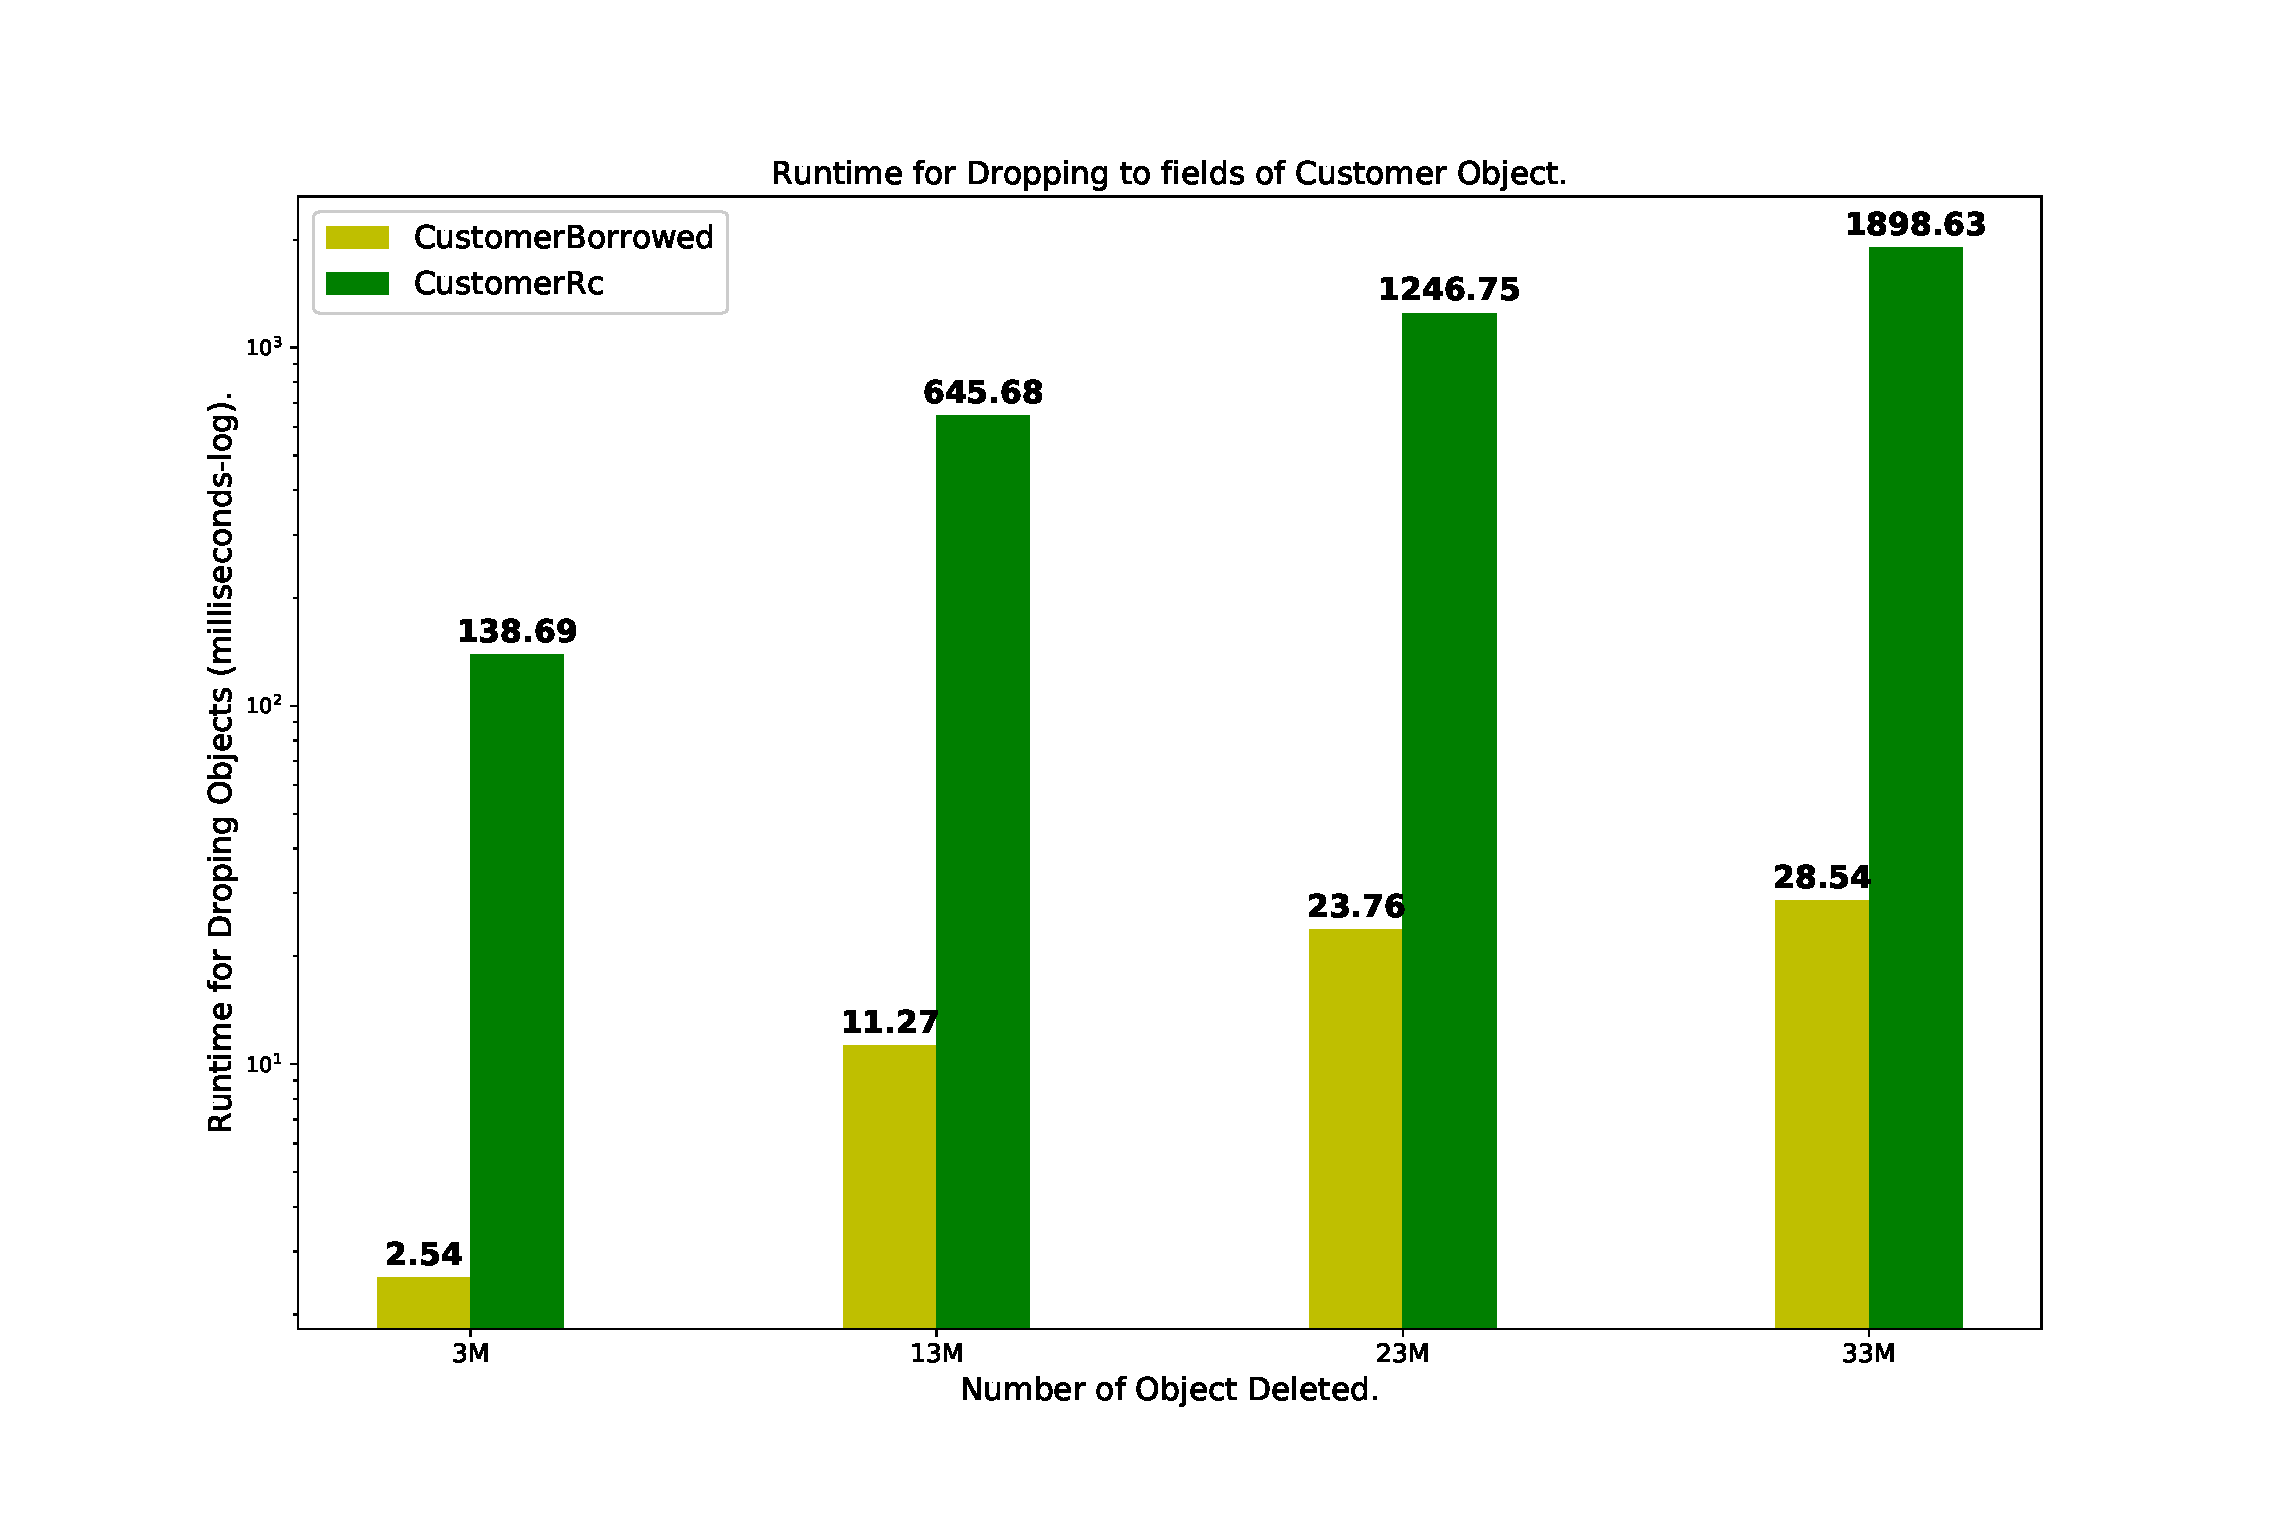
\includegraphics[width=15cm]{rust_droptime_borring_rc.eps}
    \caption{Runtime for Droping to fields of Customer Object}
    \label{fig:Sampling}
\end{figure}

\subsection{Discussion}
